%  This LaTeX template is based on T.J. Hitchman's work which is itself based on Dana Ernst's template.  
% 
% --------------------------------------------------------------
% Skip this stuff, and head down to where it says "Start here"
% --------------------------------------------------------------
 
\documentclass[12pt]{article}
 
\usepackage[margin=1in]{geometry} 
\usepackage{amsmath,amsthm,amssymb}
\usepackage{graphicx}
\usepackage{mathtools}
\linespread{1.15}

\newenvironment{problem}[2][Problem]{\begin{trivlist}
\item[\hskip \labelsep {\bfseries #1}\hskip \labelsep {\bfseries #2.}]}{\end{trivlist}}

\newcommand{\beq}[1]{\begin{equation*} \begin{split} #1 \end{split} \end{equation*}}
\newcommand{\eqline}{\noalign{\smallskip} \hline \noalign{\smallskip}}

\begin{document}

% --------------------------------------------------------------
%
%                         Start here
%
% --------------------------------------------------------------

\title{Chapter 1: The Natural Numbers Exercises' Solutions} % replace with the problem you are writing up
\author{Saif Mohammed} % replace with your name
\maketitle
\begin{problem}{a}
Explain the arithmetic advantages of \( \mathbb{Z} \), as compared with \( \mathbb{N} \). How about \( \mathbb{Q} \), as compared
with \( \mathbb{Z} \)?
\end{problem}

\begin{proof}
	$\mathbb{Z}$ is closed under subtraction while $\mathbb{N}$ is not. $\mathbb{Q}$ is closed under division while $\mathbb{Z}$ is not.

\end{proof}

\begin{problem}{b}
Why isn't \( \mathbb{Z} \) well-ordered? Why isn't \( \mathbb{Q} \) well-ordered? Why isn't the set of all rational
numbers \( x \) with \( 0 \leq x \leq 1 \) well-ordered?

\end{problem}

\begin{proof}
	There are no least elements for $\mathbb{Z}$ and $\mathbb{Q}$. So they are not well-ordered. \\
	And suppose, $S = \{ x\in \mathbb{Q}: 0 \leq x \leq 1 \}$. $S$ is not well-ordered. Because some of its subsets, for example, $S' = \{ x\in S: 0 < x \leq 1 \}$ is not well-ordered.

\end{proof}

\begin{problem}{c}
Suppose we have an infinite row of dominoes, set up on end. What sort of induction
argument would convince us that knocking down the first domino will knock them all
down?

\end{problem}

\begin{proof}
	We need to show that after knocking down the first domino, it will indeed fall. Then, assuming that the consecutive \(k\)th dominoes fall for all \(k < n\), showing that the \(n\)th domino will also fall completes the induction argument.

\end{proof}

\begin{problem}{d}
Explain why any finite subset of \( \mathbb{Q} \) is well-ordered.

\end{problem}

\begin{proof}
	Any finite subset of \(\mathbb{Q}\) has a least element, and any number smaller than this least element would not be in the set. And also the subsets of those subsets also have their respective least elements. Therefore, any finite subset of \(\mathbb{Q}\) is well-ordered.

\end{proof}





\begin{problem}{1}
Prove using mathematical induction that for all positive integers \( n \),
\[
	1 + 2 + 3 + \dots + n = \frac{n(n + 1)}{2}.
\]

\end{problem}

\begin{proof}
	$1 = \frac{1(1+1)}{2}$. Hence for $n=1$, the eqn. holds true.  Let $\text{for all } k<n \in \mathbb{N}$ , this eqn. holds true:
	\[
		1 + 2 + 3 + \dots + k = \frac{k(k + 1)}{2}.
	\]
	Now
	\beq{
		1 + 2 + \dots + k + (k+1) & = \frac{k(k + 1)}{2} + (k+1) \\
		& = \frac{k(k+1)}{2} + (k+1) \\
		& = (k+1)(\frac{k}{2} + 1) \\
		& = \frac{(k+1)(k+2)}{2}
	}
	As the eqn. also holds for $k+1$ , we can conclude it holds $\text{for all } n \in \mathbb{N}$ .


\end{proof}

\begin{problem}{2}
Prove using mathematical induction that for all positive integers \(n\),
\[
	1^2 + 2^2 + 3^2 + \dots + n^2 = \frac{n(2n+1)(n+1)}{6}.
\]

\end{problem}

\begin{proof}
	$1^2 = \frac{1(2\times 1 + 1)(1+1)}{6}$ . For $n = 1$, the eqn. is true. Let, $\text{for all } k < n \in \mathbb{N}$ ,
	\[
		1^2 + 2^2 + 3^2 + \dots + k^2 = \frac{k(2k+1)(k+1)}{6}
	\]
	Now \\
	\beq{
		1^2 + 2^2 + 3^2 + \dots + k^2 + (k+1)^2 & = \frac{k(2k+1)(k+1)}{6} + (k+1)^2 \\
		& = (k+1)[\frac{k(2k+1)}{6} + (k+1)] \\
		& = (k+1)(\frac{2k^2 + 7k + 6}{6}) \\
		& = (k+1)\frac{(2k+3)(k+2)}{6} \\
		& = \frac{(k+1)(2k+3)(k+2)}{6}
	}
	Therefore, the eqn. holds $\text{for all } n \in \mathbb{N}$ .


\end{proof}

\begin{problem}{3}
You probably recall from your previous mathematical work the \textit{triangle inequality}:
for any real numbers \( x \) and \( y \),
\[
	|x + y| \leq |x| + |y|.
\]
Accept this as given (or see a calculus text to recall how it is proved). Generalize the triangle inequality, by proving that
\[
	|x_1 + x_2 + \dots + x_n| \leq |x_1| + |x_2| + \dots + |x_n|,
\]
for any positive integer \( n \).

\end{problem}

\begin{proof}
	For $n = 1, |x_1| \leq |x_1|$ is true.
	For $n = 2, |x_1 + x_2| \leq |x_1| + |x_2|$ is true. \\
	Let, $\text{for all } k < n \in \mathbb{N}$ ,
	\begin{align*}
		         & |x_1| + |x_2| + \dots + |x_k| \geq |x_1 + x_2 + \dots + x_k|                                                     \\
		\implies & |x_1| + |x_2| + \dots + |x_k| + |x_ {k+1}|\geq |z| + |x_{k+1}| \geq |z + x_{k+1}| & \text{[triangle inequality]} \\
		\implies & |x_1| + |x_2| + \dots  + |x_ {k+1}| \geq |x_1 + x_2 + \dots + x_{k+1}|
	\end{align*}
	Therefore, the generalized inequality holds for all $n \in \mathbb{N}$ .

\end{proof}

\begin{problem}{4}
Given a positive integer \( n \), recall that \( n! = 1 \cdot 2 \cdot 3 \cdot \dots \cdot n \) (this is read as \( n \) factorial).
Provide an inductive definition for \( n! \). (It is customary to actually start this definition
at \( n = 0 \), setting \( 0! = 1 \).)

\end{problem}

\begin{proof}
	Inductive definition of factorial:
	\begin{align*}
		 & 0! = 1,             \\
		 & n! = (n-1)! \cdot n
	\end{align*}

\end{proof}

\begin{problem}{5}
Prove that \( 2^n < n! \) for all \( n \geq 4 \).

\end{problem}

\begin{proof}
	For $n = 4, \; 2^4 < 4!$ holds true.
	Let, for all $k \geq 4$ and $k < n \in \mathbb{N}$,
	\begin{align*}
		         & 2^k < k!                                                                 \\
		\implies & (k+1) \cdot 2^k < k!\cdot (k+1)                                          \\
		\implies & 2\cdot 2^k < (k+1)\cdot 2^k < (k+1)! & [2 < 4 \leq k \implies 2 < k + 1] \\
		\implies & 2^{k+1} < (k+1)!
	\end{align*}

\end{proof}

\begin{problem}{6}
Prove that for all positive integers \( n \),
\[
	1^3 + 2^3 + \dots + n^3 = \left( \frac{n(n + 1)}{2} \right)^2.
\]

\end{problem}

\begin{proof}
	For $n = 1, \; 1^3 = (\frac{1(1+1)}{2})^2$ holds true.
	Let, $\text{for all } k < n \in \mathbb{N}$,
	\[
		1^3 + 2^3 + \dots + k^3 = \left( \frac{k(k + 1)}{2} \right)^2
	\]
	Now, \\
	\begin{align*}
		1^3 + 2^3 + \dots + k^3 + (k+1)^3 & = \left( \frac{k(k + 1)}{2} \right)^2 + (k+1)^3 \\
		                                  & = (k+1)^2[\frac{k^2}{4} + (k+1)]                \\
		                                  & = (k+1)^2 \cdot \frac{k^2 + 4k +4}{4}           \\
		                                  & = (k+1)^2 \cdot \frac{(k+2)^2}{4}               \\
		                                  & = \left( \frac{(k+1)(k+2)}{2} \right)^2
	\end{align*}
	Therefore, the equation holds $\text{for all } n \in \mathbb{N}$.

\end{proof}

\begin{problem}{7}
Prove the familiar geometric progression formula. Namely, suppose that \( a \) and \( r \)
are real numbers with \( r \neq 1 \). Then show that
\[
	a + ar + ar^2 + \dots + ar^{n-1} = \frac{a - a r^n}{1 - r}.
\]

\end{problem}

\begin{proof}
	For $n = 1, \; ar^{1-1} = a = \frac{a(1-r^1)}{1-r}$ .
	Let, $\text{for all } k < n \in \mathbb{N}$,
	\[
		a + ar + ar^2 + \dots + ar^{k-1} = \frac{a(1 - r^k)}{1 - r}.
	\]
	Now
	\begin{align*}
		a + ar + ar^2 + \dots + ar^{k-1} + ar^k & = a \cdot \frac{1 - r^k}{1 - r} + ar^k          \\
		                                        & = a \cdot \frac{1 - r^k + r^k - r^{k+1}}{1 - r} \\
		                                        & = \frac{a - ar^{k+1}}{1 - r}
	\end{align*}
	Therefore, the formula holds $\text{for all } n \in \mathbb{N}$.

\end{proof}

\begin{problem}{8}
Prove that for all positive integers \( n \),
\[
	\frac{1}{1 \cdot 2} + \frac{1}{2 \cdot 3} + \dots + \frac{1}{n(n + 1)} = \frac{n}{n + 1}.
\]

\end{problem}

\begin{proof}
	For $n = 1, \; \frac{1}{1 \cdot (1+1)} = \frac{1}{1 + 1}$ .
	Let, $\text{for all } k < n \in \mathbb{N}$,
	\[
		\frac{1}{1 \cdot 2} + \frac{1}{2 \cdot 3} + \dots + \frac{1}{k(k + 1)} = \frac{k}{k + 1}
	\]
	Now
	\begin{align*}
		\frac{1}{1 \cdot 2} + \frac{1}{2 \cdot 3} + \dots + \frac{1}{k(k + 1)} + \frac{1}{(k+1)(k+2)}
		 & = \frac{k}{k + 1} + \frac{1}{(k+1)(k+2)} \\
		 & = \frac{k(k+2) + 1}{(k+1)(k+2)}          \\
		 & = \frac{k^2 + 2k + 1}{(k+1)(k+2)}        \\
		 & = \frac{(k+1)^2}{(k+1)(k+2)}             \\
		 & = \frac{k + 1}{k + 2}
	\end{align*}
	Therefore, the identity given holds for all $n \in \mathbb{N}$.

\end{proof}

\begin{problem}{9}
By trial and error, try to find the smallest positive integer expressible as \( 12x + 28y \),
where \( x \) and \( y \) are allowed to be any integers.

\end{problem}

\begin{proof}
	It is obvious that 4 is expressible as $12x + 28y$ if we take $x = -2, y = 1$. So we can say that the smallest positive integer expressible as $12x + 28y$ must be in the range: $[1, 4]$. But the integer must be even because $12x + 28y$ is an addition of two even numbers. So we just have to investigate if 2 is expressible in this way.\\
	Let,
	\begin{align*}
		         & 2 = 12x + 28y \\
		\implies & 1 = 6x + 14y
	\end{align*}
	which is not possible because the parity of LHS and RHS does not match. Therefore, 4 is the desired integer.

\end{proof}

\begin{problem}{10}
A complete graph is a collection of \( n \) points, each of which is connected to every
other point. The complete graphs on 3, 4, and 5 points are illustrated below:\\
\begin{center}
	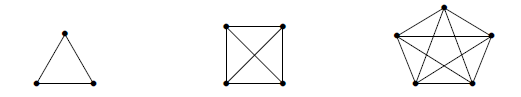
\includegraphics[width=0.5\linewidth]{image.png}
\end{center}
Use mathematical induction to prove that the complete graph on \( n \) points has exactly $\frac{n(n-1)}{2}$ lines.

\end{problem}

\begin{proof}
	For $n = 1, \; 0 = \frac{1(1-1)}{2}$. For $n = 2, \; 1 = \frac{2(2-1)}{2}$. \\
	Let, $\text{for all } k < n \in \mathbb{N}$, the complete graph on k points has exactly $\frac{k(k-1)}{2}$ lines. \\
	Now, if we add another point $((k+1)th)$, then to make the graph complete, we have to connect the other $k$ points with the newly added point. Hence, new $k$ lines will form.
	So, for $k + 1$ points,
	\begin{align*}
		\text{number of lines} & = \frac{k(k-1)}{2} + k \\
		                       & = \frac{k(k+1)}{2}
	\end{align*}
	Therefore, we can conclude $\text{for all } n \in \mathbb{N}$, the complete graph on $n$ points has exactly $n(n-1)/2$ lines.

\end{proof}

\begin{problem}{11}
Consider the sequence \( \{a_n\} \) defined inductively as follows:
\[
	a_1 = a_2 = 1, \quad a_{n+2} = 2a_{n+1} - a_n.
\]
Use mathematical induction to prove that \( a_n = 1 \), for all natural numbers \( n \).

\end{problem}

\begin{proof}
	For $n = 1, a_3 = 2a_2 - a_1 = 2\cdot 1 - 1 = 1$. Let, $\text{for all } k < n \in \mathbb{N}, \; a_k = 1$.\\
	Now
	\begin{align*}
		a_{k+1} & = 2a_k - a_{k-1} \\
		        & = 2\cdot 1 - 1   \\
		        & = 1
	\end{align*}

\end{proof}

\begin{problem}{12}
Consider the sequence \( \{a_n\} \) defined inductively as follows:
\[
	a_1 = 5, \quad a_2 = 7, \quad a_{n+2} = 3a_{n+1} - 2a_n.
\]
Use mathematical induction to prove that \( a_n = 3 + 2^n \), for all natural numbers \( n \).

\end{problem}

\begin{proof}
	$a_{n+2} = 3a_{n+1} - 2a_n$ can be expressed as $a_n = 3a_{n-1} - 2a_{n-2}$ .
	For $n = 1, 2, and 3, \; a_n = 3 + 2^n$. Let, $\text{for all } k < n \in \mathbb{N}, \; a_k = 3 + 2^k$. \\
	Now
	\begin{align*}
		a_{k+1} & = 3a_k - 2a_{k-1}          \\
		        & = 3(3+2^k) - 2(3+2^{k-1})  \\
		        & = 9 + 3\cdot 2^k - 6 - 2^k \\
		        & = 3 + 2\cdot 2^k           \\
		        & = 3 + 2^{k+1}
	\end{align*}

\end{proof}

\begin{problem}{13}
Consider the Fibonacci sequence \( \{a_n\} \).

\begin{itemize}
	\item[(a)] Use mathematical induction to prove that
	      \[
		      a_{n+1} a_{n-1} = (a_n)^2 + (-1)^n.
	      \]

	\item[(b)] Use mathematical induction to prove that
	      \[
		      a_n = \frac{(1 + \sqrt{5})^n - (1 - \sqrt{5})^n}{2^n \sqrt{5}}.
	      \]
\end{itemize}

\end{problem}

\begin{proof}
	(a) For $n = 1$,
	\begin{align*}
		         & a_2\cdot a_0 = a_1^2 + (-1)^1             \\
		\implies & 1\cdot 0 = a_1^2 - 1          & [a_0 = 0] \\
		\implies & a_1 = 1
	\end{align*}
	For $n = 2$,
	\begin{align*}
		         & a_3\cdot a_1 = a_2^2 + (-1)^2 \\
		\implies & a_3 \cdot 1 = 1^2 + 1         \\
		\implies & a_3 = 2
	\end{align*}
	For $n = 1 \text{ and } 2$ , the inequality holds. Let, $\text{for all } k < n \in \mathbb{N}$,
	\[
		a_{k+1}\cdot a_{k-1} = a_k^2 + (-1)^k
	\]
	Now
	\begin{align*}
		 & a_{k+2}\cdot a_k                                        \\
		 & = (a_{k+1} + a_k) \cdot a_k                             \\
		 & = a_k \cdot a_{k+1} + a_{k+1}\cdot a_{k-1} + (-1)^{k+1} \\
		 & = a_{k+1}(a_k + a_{k-1}) + (-1)^{k+1}                   \\
		 & = a_{k+1}^2 + (-1)^{k+1}
	\end{align*}
	Therefore, the identity holds true $\text{for all } n \in \mathbb{N}$.\\

	(b) For $n = 1$,
	\[
		a_1 = \frac{(1+\sqrt{5})^1 - (1-\sqrt{5})^1}{2^1\sqrt{5}}
	\]
	Let, $\text{for all } k < n \in \mathbb{N}$,
	\[
		a_k = \frac{(1+\sqrt{5})^k - (1-\sqrt{5})^k}{2^k \sqrt{5}}
	\]
	Now
	\begin{align*}
		a_{k+1} & = a_k + a_{k-1}                                                                                                                                                                                                 \\
		        & = \frac{(1+\sqrt{5})^k - (1-\sqrt{5})^k}{2^k \sqrt{5}} + \frac{(1+\sqrt{5})^{k-1} - (1-\sqrt{5})^{k-1}}{2^{k-1} \sqrt{5}}                                                                                       \\
		        & = \frac{(1+\sqrt{5})^k}{2^k \sqrt{5}} - \frac{(1-\sqrt{5})^k}{2^k \sqrt{5}} + \frac{2}{1 + \sqrt{5}}\cdot \frac{(1+\sqrt{5})^k}{2^k \sqrt{5}} - \frac{2}{1 - \sqrt{5}}\cdot \frac{(1-\sqrt{5})^k}{2^k \sqrt{5}} \\
		        & = \frac{(1+\sqrt{5})^k}{2^k \sqrt{5}} + \frac{2}{1+\sqrt{5}} \cdot \frac{(1+\sqrt{5})^k}{2^k \sqrt{5}} - \frac{(1-\sqrt{5})^k}{2^k \sqrt{5}} - \frac{2}{1 - \sqrt{5}}\cdot \frac{(1- \sqrt{5})^k}{2^k\sqrt{5}}
	\end{align*}
	Now
	\begin{align*}
		 & (1 + \sqrt{5})^k + \frac{2}{1 + \sqrt{5}}\cdot (1 + \sqrt{5})^k   \\
		 & = (1 + \sqrt{5})^k \left( 1 + \frac{2(1-\sqrt{5})}{1 - 5} \right) \\
		 & = (1 + \sqrt{5})^k (1 - \frac{1 - \sqrt{5}}{2})                   \\
		 & = (1 + \sqrt{5})^k (\frac{1 + \sqrt{5}}{2})                       \\
		 & = \frac{(1 + \sqrt{5})^{k + 1}}{2}
	\end{align*}
	Similarly,
	\begin{align*}
		 & (1 - \sqrt{5})^k + \frac{2}{1 - \sqrt{5}}\cdot (1 - \sqrt{5})^k \\
		 & = \frac{(1 - \sqrt{5})^{k+1}}{2}
	\end{align*}
	Finally,
	\begin{align*}
		 & \frac{1}{2^k \sqrt{5}}[\frac{(1 + \sqrt{5})^{k+1}}{2} - \frac{(1 - \sqrt{5})^{k+1}}{2}] \\
		 & = \frac{(1 + \sqrt{5})^{k+1} - (1 - \sqrt{5})^{k+1}}{2^{k+1} \sqrt{5}}
	\end{align*}
	Therefore, the formula holds $\text{for all } n \in \mathbb{N}$.

\end{proof}

\begin{problem}{14}
In this problem you will prove some results about the binomial coefficients, using
induction. Recall that
\[
	\binom{n}{k} = \frac{n!}{(n - k)!k!},
\]
where \( n \) is a positive integer, and \( 0 \leq k \leq n \).

\begin{itemize}
	\item[(a)] Prove that
	      \[
		      \binom{n}{k} = \binom{n-1}{k} + \binom{n-1}{k-1},
	      \]
	      for \( n \geq 2 \) and \( k < n \). \textbf{Hint:} You do not need induction to prove this. Bear in mind
	      that \( 0! = 1 \).

	\item[(b)] Verify that
	      $
		      \binom{n}{0} = 1 \quad \text{and} \quad \binom{n}{n} = 1.
	      $
	      Use these facts, together with part (a), to prove
	      by induction on \( n \) that \( \binom{n}{k} \) is an integer, for all \( k \) with \( 0 \leq k \leq n \). \textbf{(Note:} You
	      may have encountered \( \binom{n}{k} \) as the count of the number of \( k \)-element subsets of a
	      set of \( n \) objects; it follows from this that \( \binom{n}{k} \) is an integer. What we are asking
	      for here is an inductive proof based on algebra.)

	\item[(c)] Use part (a) and induction to prove the \textbf{Binomial Theorem}: For non-negative
	      \( n \) and variables \( x, y \),
	      \[
		      (x + y)^n = \sum_{k=0}^{n} \binom{n}{k} x^{n-k} y^k.
	      \]
\end{itemize}

\end{problem}

\begin{proof}
	(a) \begin{align*}
		\binom{n -1}{k} + \binom{n - 1}{k - 1}
		 & = \frac{(n-1)!}{(n-k-1)!k!} + \frac{(n-1)!}{(n-k)!(k-1)!}                                     \\
		 & = (n-1)! \left( \frac{1}{(n-k-1)!(k-1)!\cdot k} + \frac{1}{(n-k)\cdot (n-k-1)!(k-1)!} \right) \\
		 & = (n-1)!\cdot \frac{n-k+k}{(n-k)\cdot (n-k-1)! k\cdot (k-1)!}                                 \\
		 & = \frac{n!}{(n-k)!k!}                                                                         \\
		 & = \binom{n}{k}
	\end{align*}

	(b) $\binom{n}{0} = \frac{n!}{(n-0)!0!} = \frac{n!}{n!\cdot 1} = 1$. $\binom{n}{n} = \frac{n!}{(n-n)!n!} = \frac{n!}{0!n!} = 1$.\\
	For $n = 1, \; \binom{1}{k} = 1 \text{, where } 0 \leq k \leq 1$, which is an integer. Let, $\text{for all } x < n \in \mathbb{N}, \binom{x}{k} \text{, where } 0 \leq k \leq x$, is an integer. \\
	Now If $k = 0, \binom{x + 1}{0} = 1$. If $k = x + 1, \binom{x + 1}{x + 1} = 1$.
	If $k < x + 1$,
	\[
		\binom{x + 1}{k} = \binom{x}{k} + \binom{x}{k - 1}.
	\]
	Both $\binom{x}{k}$ and $\binom{x}{k - 1}$ are in integers. Hence, their addition is also an integer. Therefore, we conclude $\binom{n}{k}$, where $0 \leq \text{for all } k \leq n$, is an integer.

	(c) For $n = 0, \; (x + y)^0 = 1 = \binom{0}{0}x^{0-0}y^0$. Let, $\text{for all } m < n \in {\mathbb{N}} \cup \{0\}$,
	\[
		(x + y)^m = \sum_{k=0}^{m} \binom{m}{k} x^{m-k} y^k
	\]
	Now
	\begin{align*}
		 & (x + y)^{m+1} = (x+y)(x+y)^m                                                         \\
		 & = \sum_{k=0}^m \binom{m}{k}x^{m+1-k}y^{k} + \sum_{k=0}^m \binom{m}{k} x^{m-k}y^{k+1}
	\end{align*}
	Separating the two terms:
	\begin{align}
		\sum_{k=0}^m \binom{m}{k} x^{m+1-k} y^k = \binom{m}{0} x^{m+1} y^0 + \sum_{k=1}^m \binom{m}{k} x^{m+1-k} y^k \\
		\sum_{k=0}^m \binom{m}{k} x^{m-k} y^{k+1} = \sum_{k=0}^{m-1} \binom{m}{k} x^{m-k} y^{k+1} + \binom{m}{m} x^0 y^{m+1}
	\end{align}
	Taking $c-1 = k \implies c = k+1$,
	\begin{align}
		\sum_{k=0}^{m-1} \binom{m}{k} x^{m-k} y^{k+1} = \sum_{c=1}^m \binom{m}{c-1} x^{m+1-c} y^c
	\end{align}
	In (3), we can replace $c$ with $k$ as they just represents a variable.
	\begin{align}
		\sum_{c=1}^m \binom{m}{c-1} x^{m+1-c} y^c = \sum_{k=1}^m \binom{m}{k-1} x^{m+1-k} y^k
	\end{align}
	From (2) and (4),
	\begin{align}
		\sum_{k=0}^m \binom{m}{k} x^{m-k} y^{k} = \sum_{k=1}^m \binom{m}{k-1} x^{m+1-k} y^{k} + \binom{m}{m} x^0 y^{m+1}
	\end{align}
	From (1) and (5),
	\begin{align*}
		 & (x + y)^{m+1}                                                                                                                                                     \\
		 & = \binom{m}{0} x^{m+1} y^0 + \sum_{k=1}^m \left[ \binom{m}{k} + \binom{m}{k-1} \right]x^{m+1-k} y^k + \binom{m}{m} x^0 y^{m+1}                                    \\
		 & = \binom{m+1}{0} x^{m+1} y^0 + \sum_{k=1}^m \binom{m+1}{k} x^{m+1-k} y^k + \binom{m+1}{m+1} x^0 y^{m+1}                        & \text{[Using (a) and parts (b)]} \\
		 & = \sum_{k=0}^{m+1} \binom{m+1}{k} x^{m+1-k} y^k
	\end{align*}
	Therefore, Binomial Theorem works $\text{for all } n \in {\mathbb{N}}\cup \{0\}$.

\end{proof}

\begin{problem}{15}
Criticize the following `proof' showing that all cows are the same color. It suffices to show that any herd of \( n \) cows has the same color. If the herd has but one cow, then trivially all the cows in the herd have the same color. Now suppose that we have a herd of \( n \) cows and \( n > 1 \). Pick out a cow and remove it from the herd, leaving \( n - 1 \) cows; by the induction hypothesis, these cows all have the same color. Now put the cow back and remove another cow. (We can do so because \( n > 1 \).) The remaining \( n - 1 \) again must all be the same color. Hence, the first cow selected and the second cow selected have the same color as those not selected, and so the entire herd of \( n \) cows has the same color.

\end{problem}

\begin{proof}
	For \( n = 2 \), if we remove one cow, then all the cows in the herd have the same color. If we then put back the removed cow and remove the other, again all the cows in the herd have the same color. However, as there is no intermediary unselected cow, these two cows do not necessarily have the same color. Therefore, the given argument does not work for \( n = 2 \), and thus the proof is invalid.

\end{proof}

\begin{problem}{16}
Prove the converse of Theorem 1.1; that is, prove that the Principle of Mathematical Induction implies the Well-ordering Principle. (This shows that these two principles are logically equivalent, and so from an axiomatic point of view it doesn't matter which we assume is an axiom for the natural numbers.)

\end{problem}

\begin{proof}
	Suppose, $Y$ is a non-empty subset of $\mathbb{N}$, which has no least element. Obviously, $1 \not \in Y$. Let, $X$ is a subset of such that $X = \mathbb{N}\backslash Y$. As $1 \not \in Y$, then $1 \in X.$ \\
	Let, $k \in X \text{ for all } k < n \in \mathbb{N}$. Now if $n$ is in $Y$, then $n$ is the least element of $Y$. But $Y$ has no least element, thus $n \not \in Y$. And so, $n \in X$. Then $X = \mathbb{N}$. So $Y$ is an empty set, which is contradictory to our hypothesis.\\
	Therefore, Principle of Mathematical Induction implies Well-ordering Principle.

\end{proof}

\begin{problem}{17}
The Strong Principle of Mathematical Induction asserts the following. Suppose that
\( X \) is a subset of \( \mathbb{N} \) that satisfies the following two criteria:
\begin{itemize}
	\item[(a)] \( 1 \in X \), and
	\item[(b)] If \( n > 1 \) and \( n - 1 \in X \), then \( n \in X \).
\end{itemize}
Then \( X = \mathbb{N} \). Prove that the Principle of Mathematical Induction holds if and only if
the Strong Principle of Mathematical Induction does.

\end{problem}

\begin{proof}
	First let's state the Principle of Mathematical Induction: Suppose \( X \) is a subset of \( \mathbb{N} \) that satisfies the following two criteria:
	\begin{enumerate}
		\item \( 1 \in X \), and
		\item If \( k \in X \) for all \( k < n \), then \( n \in X \).
	\end{enumerate}
	Then \( X = \mathbb{N} \).\\\\
	Now we prove: If the Principle of Mathematical Induction holds, then the Strong Principle of Mathematical Induction does.\\
	Let, $X$ is a subset of $\mathbb{N}$ such that it satisfies the two criteria of the Strong Principle of Mathematical Induction. \\
	For $n = 1$, $n \in X$. For $n = 2$, $n-1 = 2-1 = 1 \in X$, then $2 \in X$. {[by (b)]}\\
	Let, $k \in X$ for all $k < n \in \mathbb{N}$. So, $n-1 \in X$. And so, $n \in X$ by (b). So, by Principle of Mathematical Induction, $X = \mathbb{N}$.\\\\
	Now we prove the converse: If the Strong Principle of Mathematical Induction holds, then the Principle of Mathematical Induction does so. \\
	Let, $X$ is a subset of $\mathbb{N}$ such that it satisfies the two criteria of the Principle of Mathematical Induction. \\
	For $n = 1, 1 \in X$. For $n = 2$, as $1 \in X$ for $1 < 2$, then $2 \in X$. {[by (2)]} \\
	Suppose, $Y = \{ x\in \mathbb{N} : k\in X \text{ for all } k \leq x \}$. As $1\in X \text{ and } 1 \leq 1, 1\in Y$.\\
	Let, for $n>1, n-1 \in Y$. That means, $k \in X \text{ for all } k \leq n-1$. Now by (2), $n\in X \implies n\in Y$. So, by Strong Principle of Mathematical Induction, $Y = \mathbb{N}$ and consequently, $X = \mathbb{N}$.

\end{proof}














% --------------------------------------------------------------
%     You don't have to mess with anything below this line.
% --------------------------------------------------------------

\end{document}